% \levelB{Hardware}
The experiments did not take advantage of GPU acceleration and were  conducted on a single computer with 256GB of RAM and with 2 Intel\textregistered Xeon\textregistered E5-2630 v2 processors, with 6 cores each, with 2 hyper-threads per core, or 24 hyper-threads in total. 


% \levelB{Software}
The main software and frameworks used to build the experiments were Python 3.6 \cite{rossum_python_2019}, Jupyter notebook \cite{perez_jupyter_2019}, Tensorflow 1.14.0 \cite{google_brain_tensorflow_2019}, Keras 2.2.4-tf \cite{chollet_keras_2019}, and Fedora Linux 27.
% repository
The source code for the experiments is available at \sloppy\url{http://github.com/atilaromero/carving-experiments}.

\levelC{Accuracy vs. number of classes}

% decrease in accuracy
Figure \ref{fig:nclasses} shows the graph of accuracy versus number of classes.  Each of those points is a model trained with the indicated number of classes. The class for a block sample is the file extension of the original file. The classes/extensions used to train each model were taken at random. The bottom line indicates for comparison how accurate a random guess classifier would be. The points for two classes use transparency to improve visualization, as many of them are too close. For 2 classes, the accuracy values are between 0.5 and 1.0, with a greater concentration near 1.0. For 28 classes, the accuracy values are between 0.55 and 0.58.

The lines ``hard file types first'' and ``easy file types first'' were created by selecting the file types that would compose the dataset. The selection was based on the results described in the next subsection, ``Accuracy of pairs of classes'', ordering the file types by their minimum accuracy values and following this order to choose file types. For example, the ``hard file types first'' point for three classes was obtained by training a model with the file types ``pps'', ``ppt'', and ``gz'', the three classes with lower minima in Figure \ref{fig:dual}.

\noindent
\begin{figure*}[htb!]
\centering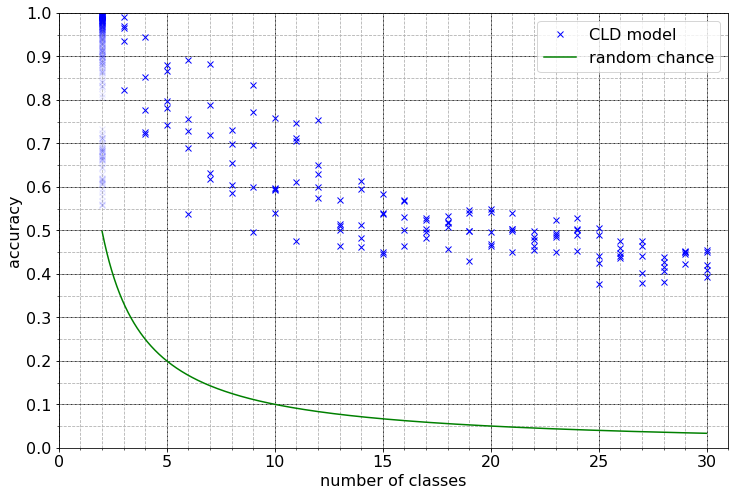
\includegraphics[width=0.8\textwidth]{content/nclasses.png}
\caption{\label{fig:nclasses}Validation accuracy by number of classes}%
\end{figure*}

\levelC{Accuracy of pairs of classes}

Figure \ref{fig:dual} shows the graph of the accuracy of each class when compared individually with each one of the others, resulting in 378 models, one for each possible pair of classes. File types where all the points are close to 1.0 are hardly mistaken for other types, while file types presenting accuracy values close to 0.5 can be mistaken for other file types by the model.

\noindent
\begin{figure*}[htb!]
\centering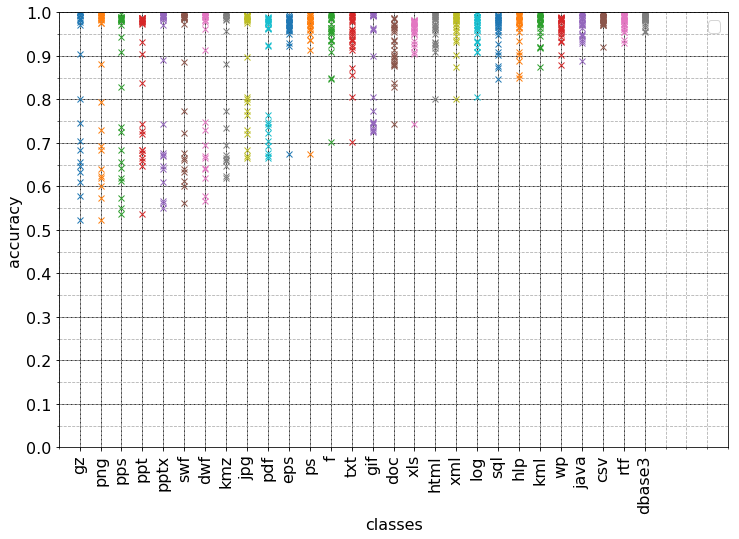
\includegraphics[width=0.8\textwidth]{content/dual.png}
\caption{\label{fig:dual}Validation accuracy of models trained with pair of classes}%
\end{figure*}

\levelC{PCA}

A 28x28 matrix was made using the accuracy of the models built for each pair of classes as a distance measure. A PCA dimensionality reduction technique was used to plot this data in a 2D graph, grouping similar file types. The result is shown in figures \ref{fig:pca} and \ref{fig:pca2}. Similar file types are next to each other, while those that can be easily distinguished by the models are represented by points that are distant from each other.

\noindent
\begin{figure*}[htb!]
\centering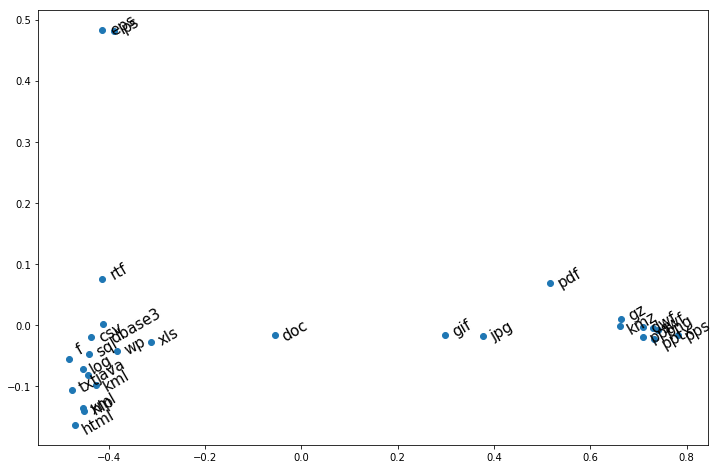
\includegraphics[width=0.8\textwidth]{content/pca.png}
\caption{\label{fig:pca}PCA of accuracy of models trained with pair of classes}%
\end{figure*}


\noindent
\begin{figure*}[htb!]
\centering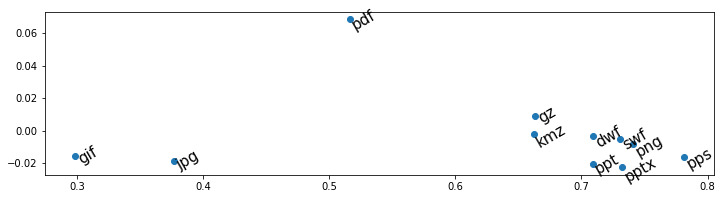
\includegraphics[width=0.8\textwidth]{content/pca2.png}
\caption[PCA of accuracy of models trained with pair of classes - detail]{\label{fig:pca2}PCA of accuracy of models trained with pair of classes - lower right detail}%
\end{figure*}

% the problem of unseen file types
% \levelC{Limitations and threats to validity}
